\documentclass[12pt]{article}

\usepackage{amsmath,mathtools,amssymb}
\usepackage{hyperref} 
\usepackage{listings}
\usepackage{courier}
\usepackage{graphicx,url}
\usepackage{color}
\usepackage{xcolor}
\usepackage{wasysym}
\usepackage{soul}
\usepackage{textcomp}

\graphicspath{{../figs/}}

\newcommand{\dash}{\textemdash}
\newcommand{\mono}[1]{\texttt{#1}}
\newcommand{\type}[1]{\textcolor{purple}{\mono{#1}}}
\newcommand{\mb}[1]{\mathbf{#1}}
\newcommand{\inter}[0]{\[\photon\]\\}

\newcommand{\spm}[1]{\mono{\_\_#1\_\_}}

\usepackage[brazil]{babel}  
\usepackage[utf8]{inputenc}

\title{Lista Extra de Computação \\ {\normalsize DCC / UFRJ}}
\author{Pedro Maciel Xavier (monitor)\\ \mono{pedromxavier@poli.ufrj.br}}
\begin{document}
	\maketitle
	\section*{Introdução}
	\dash "Fala galerinha do YouTube!"\\
	Essa lista de exercícios tenta cobrir toda a matéria dos cursos de Computação da UFRJ e ainda se encontra em desenvolvimento. A intenção é que ela tenha um gabarito bem aberto, deixando muito das respostas pra criatividade do aluno. As questões são, em geral, grandes para se resolver e podem necessitar de alguma pesquisa adicional. Elas tem estrelinhas $\star$ indicando a dificuldade estimada. Alguns exercícios foram inspirados em outros propostos nos materiais dos professores que estão devidamente citados no final. É importante você tire suas dúvidas e dê um retorno do que achou dos exercícios através do \mono{e-mail} no cabeçalho.
	\\ \\
	Boa diversão!
	\pagebreak
	
	\section{Orientação a Objeto (Classes)}
	\subsection{O Bidicionário \cite{asad} $\star$}
	Todos conhecemos os dicionários do \mono{Python}, que guardam diversos objetos em pares da forma \mono{"chave":valor}. Vejamos um exemplo:
	\begin{verbatim}
	>>> casa = {'quartos':4, 'banheiros':5, 'andares':3, 'm^2':210}
	>>> casa['quartos']
	4 
	\end{verbatim}
	O objetivo deste exercício é criar um dicionário de mão dupla! Tudo que você precisa fazer é sobrescrever o método \spm{setitem} em um novo tipo que herda as propriedades de um dicionário comum do \mono{Python}, o \type{dict}. Basta completar o exemplo abaixo!
	\begin{verbatim}
	class Bidict(dict):
	    def __init__(self, mapping={}):
	        dict.__init__(self, mapping)
	    ...
	>>> bd = Bidict()
	>>> bd["a"] = 4
	>>> bd[3] = "d"
	>>> print bd
	{"a":4, 4:"a", 3:"d", "d":3}
	\end{verbatim}
	Lembrando que se um objeto não puder ser chave de um dicionário, ele também não poderá ser um valor do bidicionário!
	
		\subsection{Ora Bolas! $\star$}
	Agora você tem que fazer o seguinte: Crie uma classe chamada \mono{Bola} que deve implementar objetos com as seguintes características:
	\begin{enumerate}
		\item O raio nominal da bola.
		\item A pressão de ar máxima (em $bar$).
		\item A pressão de ar atual. (em $bar$).
		\item A condição da bola (furada ou não).
		\item Uma onomatopeia correspondente ao barulho que a bola faz quando quica, e outra para caso ela fure.
		\item A probabilidade da bola furar quando quica.
	\end{enumerate}
	Além disso, tendo uma bola em mãos você deve poder:
	\begin{enumerate}
		\item Quicar! Caso ela não esteja vazia.
		\item Encher em alguma quantidade de $bar$, passada como argumento da função, caso ela não esteja furada. Se você encher de mais ela deve furar!
		\item Calcular o seu volume.
	\end{enumerate}
	Feita a bola, você deve criar uma classe \mono{BolaQuadrada} que herde as propriedades de uma bola comum, mas tenha as adaptações necessárias para o seu formato. Ela deve, por exemplo, ter $50\%$ de chance de quicar em uma tentativa.
	\\ \\
	Faça também a classe \mono{BolaDeFesta}, que deve furar sempre que quicar. Dê a ela um som de estouro interessante.
	
	\subsection{Frações $\star$}
	Um número racional $r \in \mathbb{Q}$ é aquele que pode ser escrito como: 
	\[r = \frac{p}{q} ; p,q \in \mathbb{Z} ; q \neq 0\]
	Crie uma classe \mono{Fracao} que implemente as seguintes operações e métodos:
	\begin{enumerate}
		\item Um método que simplifique a fração.
		\item \mono{+}, \mono{-}, \mono{*}, \mono{**} e \mono{/}.
		\item \mono{-} (\spm{neg}) e \mono{\texttildelow} (\spm{invert}).
		\item \spm{repr} que retorna \mono{"p|q"}.
		\item \spm{float}, que calcula a divisão em ponto-flutuante.
	\end{enumerate}

	\begin{verbatim}
	class Fracao(object):
	    
	    def __init__(self, p, q):
	        assert type(p) is int
	        assert type(q) is int
	        assert q != 0
	        ...
	        
	\end{verbatim}
	
	\subsection{Polinômios \cite{esperanca} $\star\star$}
	Um polinômio de grau $n$ é aquele da forma
	\[p(x) = \sum_{i=0}^{n} a_{i} x^{i}=a_{0} + a_{1}x + \dots + a_{n} x^{n}.\]
	Sabendo isso, faça uma classe \mono{Polinomio} que implemente:
	\begin{enumerate}
		\item A definição de um coeficiente do polinômio através do método \spm{setitem}, ou seja, \mono{p[2] = 3} faria com que o coeficiente $a_{2}$ do polinômio $p$ tivesse valor $3$.
		
		\item O cálculo do grau do polinômio $p$, que deve ser retornado quando chamamos \type{len}\mono{(p)}.
		
		\item A soma, a subtração e a multiplicação usual de polinômios usando os operadores da linguagem (\mono{+},\mono{-},\mono{*}), que deve retornar um novo objeto da classe \mono{Polinomio}.
		
		\item E por fim, a avaliação da função num ponto $x$, usando o método especial \spm{call}.
	\end{enumerate}
	Bônus:
	\begin{enumerate}
		\item O método especial \spm{repr} que deve retornar uma \type{string} que represente o polinômio $2 + x + 3x^{2}$ na forma \mono{"2x\^{}0 + 1x\^{}1 + 3x\^{}2"}, por exemplo.
		\item Duas funções, \mono{Polinomio.integral} e \mono{Polinomio.derivada} que retornem os respectivos polinômios resultantes destas operações.
		
		\item Divisão de polinômios (\mono{f/g} e \mono{f\%g}) , que devem retornar respectivamente o quociente $q(x)$ e o resto $r(x)$ tais que $f(x) = g(x) q(x) + r(x)$.
	\end{enumerate}
	
	\subsection{Grupos $\star\star\star$}
	
	\[\photon\]
	
	\subsubsection{Interlúdio: Conjuntos}
	No \mono{Python} temos um tipo muito bacana, mas muito mesmo, chamado \type{set}. Esse carinha simula um conjunto do ponto de vista matemático, ou seja, é uma coleção de objetos distintos. Um \type{set} pode ser criado usando-se outro objeto ou informando os elementos entre colchetes:
	
	\begin{verbatim}
	>>> A = set([1,2,3])
	>>> B = {x for x in range(2,5)}
	>>> A
	set([1, 2, 3])
	>>> B
	set([2, 3, 4])
	>>> A - B
	set([1])
	>>> A | B
	set([1, 2, 3, 4])
	\end{verbatim}
	
	O \type{set} permite realizar diversas operações entre conjuntos, sendo as mais importantes: a diferença (\mono{-}), a união (\mono{|}, \emph{ou binário}) e a interseção (\mono{\&}, \emph{e binário}). 
	
	\[\photon\]\\
	
	Em Álgebra, um Grupo $G = (A, \ast)$ é formado por um conjunto $A$ e uma operação qualquer $\ast$, quando valem as seguintes regras:
	
	\begin{enumerate}
		\item $(a \ast b) \in A \,\,\, \forall a,b \in A$ [O grupo é fechado para a operação.]
		\item $\exists \, e \in A : e \ast a = a \ast e = a \,\,\, \forall a \in A$ [Existe o elemento neutro.]
		\item $\exists \, a^{-1} \in A : a \ast a^{-1} = a^{-1} \ast a = e \,\,\, \forall a \in A$ [Existe o elemento inverso.]\\
	\end{enumerate}
	Construa um objeto \mono{Grupo} que herda as características do \type{set}. Devem ser passados ao construtor: os elementos em uma coleção \mono{A}, e uma função \mono{f(a,b)} que realiza a operação $\ast$ sobre dois elementos do Grupo.
	
	\begin{verbatim}
	def f(a,b):
	    return (a + b) % 5
	    
	class Grupo(set):
	    def __init__(self, A, f):
	        ...

	    def __hash__(self):
	        return hash(tuple(self))
	        
	>>> G = Grupo([0,1,2,3,4], f)
	>>> G
	{0, 1, 2, 3, 4}
	>>> H = Grupo([0,1,2], f)
	Traceback (most recent call last):
	    File "<pyshell#1>", line 1, in <module>
	        raise Exception('Isso não é grupo!')
	Exception: Isso não é grupo!
	\end{verbatim}
	Sabido isso:
	\begin{enumerate}
		\item O construtor deve criar um erro quando as regras de Grupo não forem atendidas.
		\item A visualização do grupo mostre os elementos entre colchetes usando o método \spm{repr}.
	\end{enumerate}

	\subsection{Subparte I: Produto}
	O produto entre dois grupos é dado da seguinte forma:
	\[GH := \{g \ast h : g \in G, h\in H\} \]
	Defina o método \spm{mul} para atender a esse propósito.
	
	\subsubsection{Subparte II: Quociente}
	Existe uma operação entre grupos chamada \emph{quociente} definida por:
	\[G/H := \{gH : g \in G\} = \{\{g \ast h: h \in H\} : g \in G\}\]
	Essa operação deve retornar um \emph{conjunto de grupos} e isso só é possível se o método \spm{hash} estiver definido como no modelo. Implemente essa operação usando o método \spm{div}.
	
	\subsubsection{Subparte III: Subgrupos}
	Um Subgrupo $H$ de um Grupo $G$, que escrevemos $H < G$, é aquele cujo conjunto é subconjunto de $G$ e é $H$ também um Grupo. O tipo \type{set} já implementa os operadores \mono{>}, \mono{>=}, \mono{<}, \mono{<=} e \mono{==} comparando dois objetos do ponto de vista dos conjuntos. Reescreva os métodos \spm{gt}, \spm{ge}, \spm{lt}, \spm{le} e \spm{eq}, respectivamente, para dizer verificar, por exemplo, se \mono{H} é subgrupo de \mono{G} através da expressão \mono{H < G}.
	Feito isso, construa um método da classe \mono{Grupo} que retorne um conjunto contendo todos os subgrupos de um grupo \mono{G}.\\
	\\
	\st{Dica} Teorema: \\
	O \emph{Teorema de Lagrange} diz que sendo $G$ um grupo finito e $H$ um subgrupo de $G$, a ordem de $H$ divide a ordem de $G$.
	\[H < G \implies |G| = |H| \cdot k, k \in \mathbb{N}\]
	A ordem de um grupo $G$, escrita como $|G|$, é simplesmente o número de elementos em $G$, que pode ser obtida diretamente pela expressão \type{len}\mono{(G)}.
	
	\pagebreak
	
	\subsection{Musical $\star\star\star\star$}
	A nota \emph{lá} (A$4$) na musica ocidental corresponde a frequência de $440 Hz$. A partir desta nota podemos conhecer todas as outras frequências usando a simples fórmula:
	\[f(n) = 440 \times \sqrt[12]{2^{n}}\]
	A escala musical \emph{cromática} é dividida em $12$ semitons, cada um correspondente a uma nota:\\
	\\
	\mono{..., fá\#[-3], sol[-2], sol\#[-1], lá[0], lá\#[1], si[2],}\\ \mono{dó[3], dó\#[4], ré[5], ré\#[6], mi[7], fá[8], fá\#[9]...}\\
	\\
	Essa sequência se repete nos dois sentidos e símbolo \# lê-se \emph{sustenido}. Assim, se queremos a frequência de um \emph{dó} logo após o \emph{lá} central (A$4$), basta calcular $f(3) \approx 523.25 Hz$.\\
	Note que se temos alguma nota cuja frequência é $f(\bar{n})$, ao avançarmos $12$ semitons na escala cromática voltamos para a mesma nota, mas com frequência $f(\bar{n} + 12)$. Ao tirar a razão entre as duas frequências:
	\[\frac{f(\bar{n} + 12)}{f(\bar{n})} = \frac{440 \times \sqrt[12]{2^{\bar{n} + 12}}}{440 \times \sqrt[12]{2^{\bar{n}}}} = 2\]
	Isso nos diz que cada vez que avançamos até a próxima repetição de uma nota, dobramos a frequência! Na escala de \emph{dó maior}, que todos sabemos de cor, isso equivale a avançar uma \emph{oitava acima}.
	
	\subsubsection{Interlúdio: \mono{Beep}}
	\inter
	Um jeito fácil de fazer barulho no computador é usando a função \mono{Beep}. Se você usa o \mono{Python} no \mono{Windows} boas notícias: você só vai precisar importar a função \mono{Beep} do módulo \mono{winsound}.\\
	\\
	\mono{>>> Beep(440, 1000)}
	\begin{verbatim}
	# windows
	from winsound import Beep
	\end{verbatim}
	Pra turminha do \mono{Linux}, que precisa construir a função: \\
	\mono{\$ sudo apt-get install beep}
	\begin{verbatim}
	# linux
	import os
	def Beep(f, ms):
	    os.system("beep -f %i -l %i" % (f, ms))
	\end{verbatim}
	\inter
	
	Vamos construir agora um sensacional tocador de músicas! Você deve fazer duas classes: \mono{Som} e \mono{Musica} conforme os protótipos a seguir:
	
	\begin{verbatim}
	class Som(object):
	
	    def __init__(self, nota, duracao):
	        ...
	        
	class Musica(list):
	
	    def __init__(self, partitura, tempo, nome="",autor=""):
	        ...
	        
	    def __repr__(self):
	        # mostra "<nome>", <autor> (<tempo> bps)
	        ...
	        
	    def __call__(self):
	        # toca a musica
	        ...
	\end{verbatim}
	Um \mono{Som} deve ter:
	\begin{enumerate}
		\item O número da nota (\emph{lá}=0, \emph{si}=2, ...), que será usado para calcular a frequência dela.
		\item A duração da nota, que deve ser uma fração da \emph{batida} que seja potência de $\frac{1}{2}$. Você pode até informar somente o expoente $m$ de $(\frac{1}{2})^{m}$, onde $m \in [-2, 6]$.
	\end{enumerate}
	A duração absoluta da nota dependerá da música em que o \mono{Som} será tocado.
	\\ \\
	Já uma instância de \mono{Musica} deve receber na construção:
	\begin{enumerate}
		\item A \mono{partitura}, que é uma lista de objetos do tipo \mono{Som}.
		\item O \mono{tempo}, dado em \emph{batidas por minuto} (bps).
	\end{enumerate}
	\mono{Musica} herda as propriedades de lista, e assim pode ser percorrida com um \mono{for}, tocando nota por nota.
	\\ \\
	Tendo essa parafernália toda em mãos, construiremos esses objetos de forma que a música seja tocada através da função \mono{Beep(f, ms)}, que recebe a frequência \mono{f} da nota e a sua duração \mono{ms} em \emph{milissegundos}.

	\subsection{Quaterniões! $\star\star\star$}
	Não contente com os números complexos ($\mathbb{C}$) da forma $z = a + b\mb{i}$, a turma da matemática trouxe pra gente um ser ainda mais esquisito: o conjunto dos \emph{Quaternions} ($\mathbb{H}$).
	
	\[	
	\begin{gathered}
	q \in \mathbb{H} \iff q = a + b \mb{i} + c \mb{j} + d \mb{k} : \, a,b,c,d \in \mathbb{R}\\
	\mb{i} \times \mb{j} = -(\mb{j} \times \mb{i}) = \mb{k}\\
	\mb{j} \times \mb{k} = -(\mb{k} \times \mb{j}) = \mb{i}\\
	\mb{k} \times \mb{i} = -(\mb{i} \times \mb{k}) = \mb{j}\\
	\mb{i} \times \mb{j} \times \mb{k} = -1 \nonumber	
	\end{gathered}
	\]
	\\
	Com regras de soma convencionais, similares aos números reais e complexos, mas com uma multiplicação que mais parece o produto externo entre vetores, implemente uma classe \mono{Quaternion}, que é criada a partir dos seus $4$ coeficientes reais e implementa:
	\begin{enumerate}
		\item O operador de soma \mono{+} (\spm{add})
		\item A subtração \mono{-} (\spm{sub})
		\item A multiplicação \mono{*} (\spm{mul})
		\item O método \spm{repr} que imprima na tela, pra $q = 3 + 4\mb{j} - 2\mb{k}$ a \type{string} \mono{(3.00) + (0.00)i + (4.00)j + (-2.00)k}
	\end{enumerate}
	
	Extra:
	\begin{enumerate}
		\item O módulo do quaternião, através da função \type{abs}(q), implementada pelo método especial \spm{abs}
		\item A divisão \mono{\slash} (\spm{div})
	\end{enumerate}

	Dica:
	Implemente os métodos \spm{invert} e \spm{neg} para auxiliar na definição de \spm{div} e \spm{sub}, respectivamente.
	
	\pagebreak
	
	\section{Interface Gráfica}
	\subsection{O Triângulo de Sierpinsky $\star\star$}
	A figura a seguir chama-se \emph{Triângulo de Sierpinsky}:
	\\
	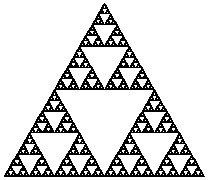
\includegraphics[height=200pt]{sierpinsky.png}
	\\
	Ela é composta por triângulos equiláteros dispostos de forma que cada triângulo contém três outros em seu interior, cada um com $\frac{1}{3}$ do lado do triângulo original.
	Desenhe essa estrutura usando o \mono{Tkinter} ou o \mono{turtle}, assim como uma função para compôr a figura de forma recursiva.
	\subsection{O Método de Monte Carlo $\star\star$}
	O Método de \emph{Monte Carlo} funciona da seguinte forma: Se temos uma determinada região e queremos calcular sua área, basta fazer com que ela esteja contida em uma outra região cuja área é conhecida. Em seguida, sorteamos pontos aleatórios $P_{i} = (x_{i}, y_{i})$ e contamos quantos pontos caem dentro da região que estamos avaliando. Assim:
	\\
	\[
	\frac{A_{figura}}{A_{total}} \approx \frac{P_{dentro}}{P_{total}} \to A_{figura} \approx \frac{P_{dentro}}{P_{total}} \times A_{total}
	\]
	\\
	Queremos então calcular a área de um círculo cujo raio é $1$. Sabemos de antemão que valor da área é $\pi$, e vamos então usar o método acima para estimar o seu valor numérico.
	\\
	\\
	Faça duas janelas usando o \mono{Tkinter}. A primeira mostra onde os pontos estão sendo posicionados, colorindo os que caem dentro de \textcolor{blue}{azul} e os que caem fora de \textcolor{red}{vermelho}. Na segunda tela, mostre em tempo real a aproximação para a área em azul conforme os pontos vão sendo posicionados. 
	\\
	\\
	\\
	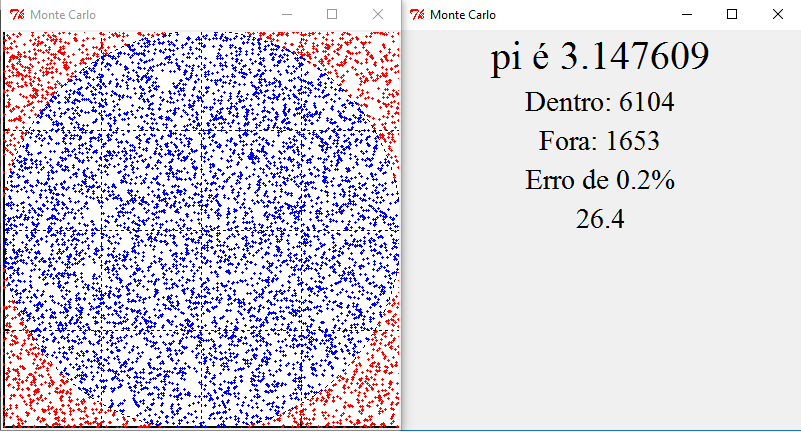
\includegraphics[height=210pt]{monte_carlo.png}
	\\
	dica: use o módulo \mono{random} para sortear os pontos!
	
	\subsection{A proporção áurea $\star\star$}
	\[0\ 1\ 1\ 2\ 3\ 5\ 8\ 13\ 21\ 34\ 55\ 89\ ... \]	
	Muitos conhecem esse conjunto de números, a famosa \emph{Sequência de Fibonacci}, que tem seu $n$-ésimo número definido por:
	\[F_{n} = F_{n-1} + F_{n-2}\]
	\[F_{0} = 0 \ e \ F_{1} = 1\]
	Se tomamos a razão entre dois números de \emph{Fibonacci} consecutivos obtemos, no limite, um número que já era conhecido pelos gregos como símbolo da beleza e da perfeição da natureza.
	\[\varphi = \lim_{n \to \infty} \frac{F_{n+1}}{F_{n}}= \frac{1+\sqrt{5}}{2} \]
	Sabido isso, sua tarefa é gerar a figura abaixo, usando o módulo que preferir, mas de forma recursiva. Para que os gregos realmente fiquem contentes com a majestade da sua figura é preciso que ela esteja conforme a proporção dada por $\varphi$.\\\\
	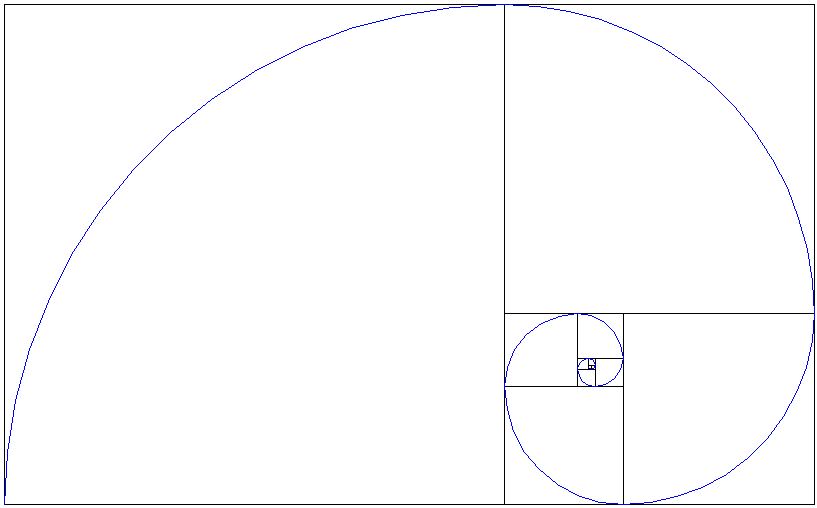
\includegraphics[height=200pt]{golden_ratio.png}
	
	\subsection{O Piano $\star\star\star$}
	O Desafio agora é pegar os resultados da Questão {\bf Musical} e construir um Piano Virtual com o \mono{Tkinter}! Desenhe as teclas em um \mono{Canvas} e use o método \mono{Canvas.bind} para associar letras como \mono{a,s,d,f,g,h,j} e \mono{k} às teclas brancas e \mono{w,e,t,y} e \mono{u} às pretas, por exemplo.
	
	\begin{thebibliography}{99}
	%\bibitem{lcarvalho} Prof. Leonardo Carvalho (2015)
	\bibitem{asad} Prof. Pedro Asad (2016)
	\bibitem{esperanca} Prof. Claudio Esperança (2018)
	\end{thebibliography}
\end{document}